\chapter{Image recognition for IBD reconstruction with the SPMT system}
\label{sec:jcnn}

As explained in chapter \ref{sec:juno}, JUNO is an experiment composed of two systems, the Large Photo Tube Multiplier (LPMT) and the Small Photo Multiplier Tubes (SPMT). Both of the system observe the same physics event inside of the same medium but they differ in their photo-coverage, respectively 75.2\% and 2.7\%, their dynamic range, a thousands versus a few dozen, and their back-end electronics (see section \ref{sec:juno:LPMT}).

Due to their differences they are complementary and their strength and weakness. One important point the difference in expected resolution, the LPMT system outperform largely the SPMT system but is subject to effects such as saturation \cite{juno_collaboration_calibration_2021} that could bias the reconstruction, effect that the SPMT system is impervious to. Also, due to the dynamic range of the LPMT, in case of high energy and high density event such as core-collapse supernova, the LPMT system could saturate and the lack of photo-coverage become a benefit.

Thus it is important to have reconstruction and analysis combined but also dedicated to each system, taking into account the specificity. The subject of this work is to propose a machine learning algorithm for the SPMT reconstruction based on Convolutional Neural Network (CNN).

\section{Motivations}

% -------------- Plan for motivation section ----------------
%\begin{itemize}
%  \item Promise of machine learning -> Exploit raw data
%  \item Victor already done reco for SPMT
%  \item Can CNN give similar results ? Better results ?
%  \item Multiple reco methods good for reconstruction
%  \item Comparison, difference in behavior
%\end{itemize}

As explained in chapter \ref{sec:ml}, Machine Learning (ML) algorithms shine when modeling complex distribution from a given dataset. In our case, we have access to complete monte-carlo simulation of our detector to produce arbitrary large datasets that could represent multiple years of data taking. Also, due to the nature of monte-carlo simulation we have access to exact truth of the modelled event like the position, energy and nature of the particle.

One of expectation when using data-driven, and so, machine learning algorithm is that the algorithm will be able to use the entirety of the raw information, preventing any loss in precision due to miss-modeling or simplification of the underlying physic process.


Another algorithm was developed in the collaboration for energy and vertex reconstruction \cite{lebrin_towards_2022} and will serve as a performance reference in this work. The two methods will also be studied event by event to try to understand and unveil coherence or incoherence between their performances.


\section{Method and model}
% --------------- Plan for method and model -----------------
%\begin{itemize}
%  \item JUNO is an array of sensor following a quasi uniform and istropic geometric repartition -> Basically pixels -> Image
%  \item CNN is gud for image processing (cite a lot of things)
%  \item Details the architecture (Inspired from VGG 16)
%    \begin{itemize}
%      \item Convolutional layers
%      \item Pooling layers -> Twice the channels when pooling by 2 -> Keep the same "amount" of information
%      \item Dropout (introduce overtraining, maybe introduce overfitting in ML chapter ?)
%      \item Vectorization fed to FCDNN
%    \end{itemize}
%  \item Data is 240x240 images
%    \begin{itemize}
%      \item Following $\theta$ and $\phi$ distribution, explain the coordinate system of JUNO
%      \item Optimized for $\approx$ 1 SPMT/pixel
%      \item 1 Charge channel
%      \item 1 Time channel
%    \end{itemize}
%  \item Discuss data format
%    \begin{itemize}
%      \item Empty pixel ? -> $Q = 0$, $T = 0$, what does it means/says ? 0 = no signal in a way
%      \item Image distortion
%        \begin{itemize}
%          \item \textbf{Maybe speak of this in the conclusion ?} Could be done in two step:
%          \item 1. Reconstruct $\theta$ and $\phi$
%          \item 2. "Rotate" the image so the event is at the center of the image -> Prevent distortion + reconstruction E and R become pseudo rotational invariant (as they should be)
%        \end{itemize}
%      \item 1 Millions MC e+ events for training (900k for train, 50k for validation and 50k for test)
%        \begin{itemize}
%          \item MC for the moment, will need to retrain with mix of calibration data (Good question, is the CNN PID agnostic ?)
%          \item 47 IBD/day -> 1M event is 21k days of data (for reference, 6 years of data is 94k events)
%          \item Events are "optimistic"
%            \begin{itemize}
%              \item No pile-up
%              \item w/o neutrons
%              \item time window is decided by electronics
%              \item We want to reconstruct the E from $\bar{\nu_e}$
%              \item Difference between multiple E -> $E_{vis}$, $E_{rec}$, $E_k$
%            \end{itemize}
%        \end{itemize}
%    \end{itemize}
%\end{itemize}

One of simplest way to look at JUNO data is to consider the detector as an array of geometrically distributed sensors on a sphere. Their repartition is almost homogeneous, on this sphere surface providing an almost equal amount of information per unit surface on this sphere. One kind of data representation that is ordered, presenting the same property as a plane is the image, which is a bounded discrete euclidian plane.

Using this representation we can arrange the SPMTs on this plane while keeping most of the neighbouring informations. The pros and cons of this representation is detailed in section \ref{jcnn:data}.

The most common approach in machine learning for image processing and image recognition is the Convolutional Neural Network (CNN). It is widely used in research and industry \cite{simonyan_very_2015, ciresan_multi-column_2012, abbasi_convolutional_2021, maksimovic_cnns_2021} due to its strengths (see section \ref{ml:cnn}) and has proven its relevance in image processing.

\subsection{Model}

The architecture we use is derived from the VGG-16 architecture \cite{simonyan_very_2015} illustrated in figure \ref{fig:jcnn:vgg16}

\begin{figure}[ht]
  \centering
  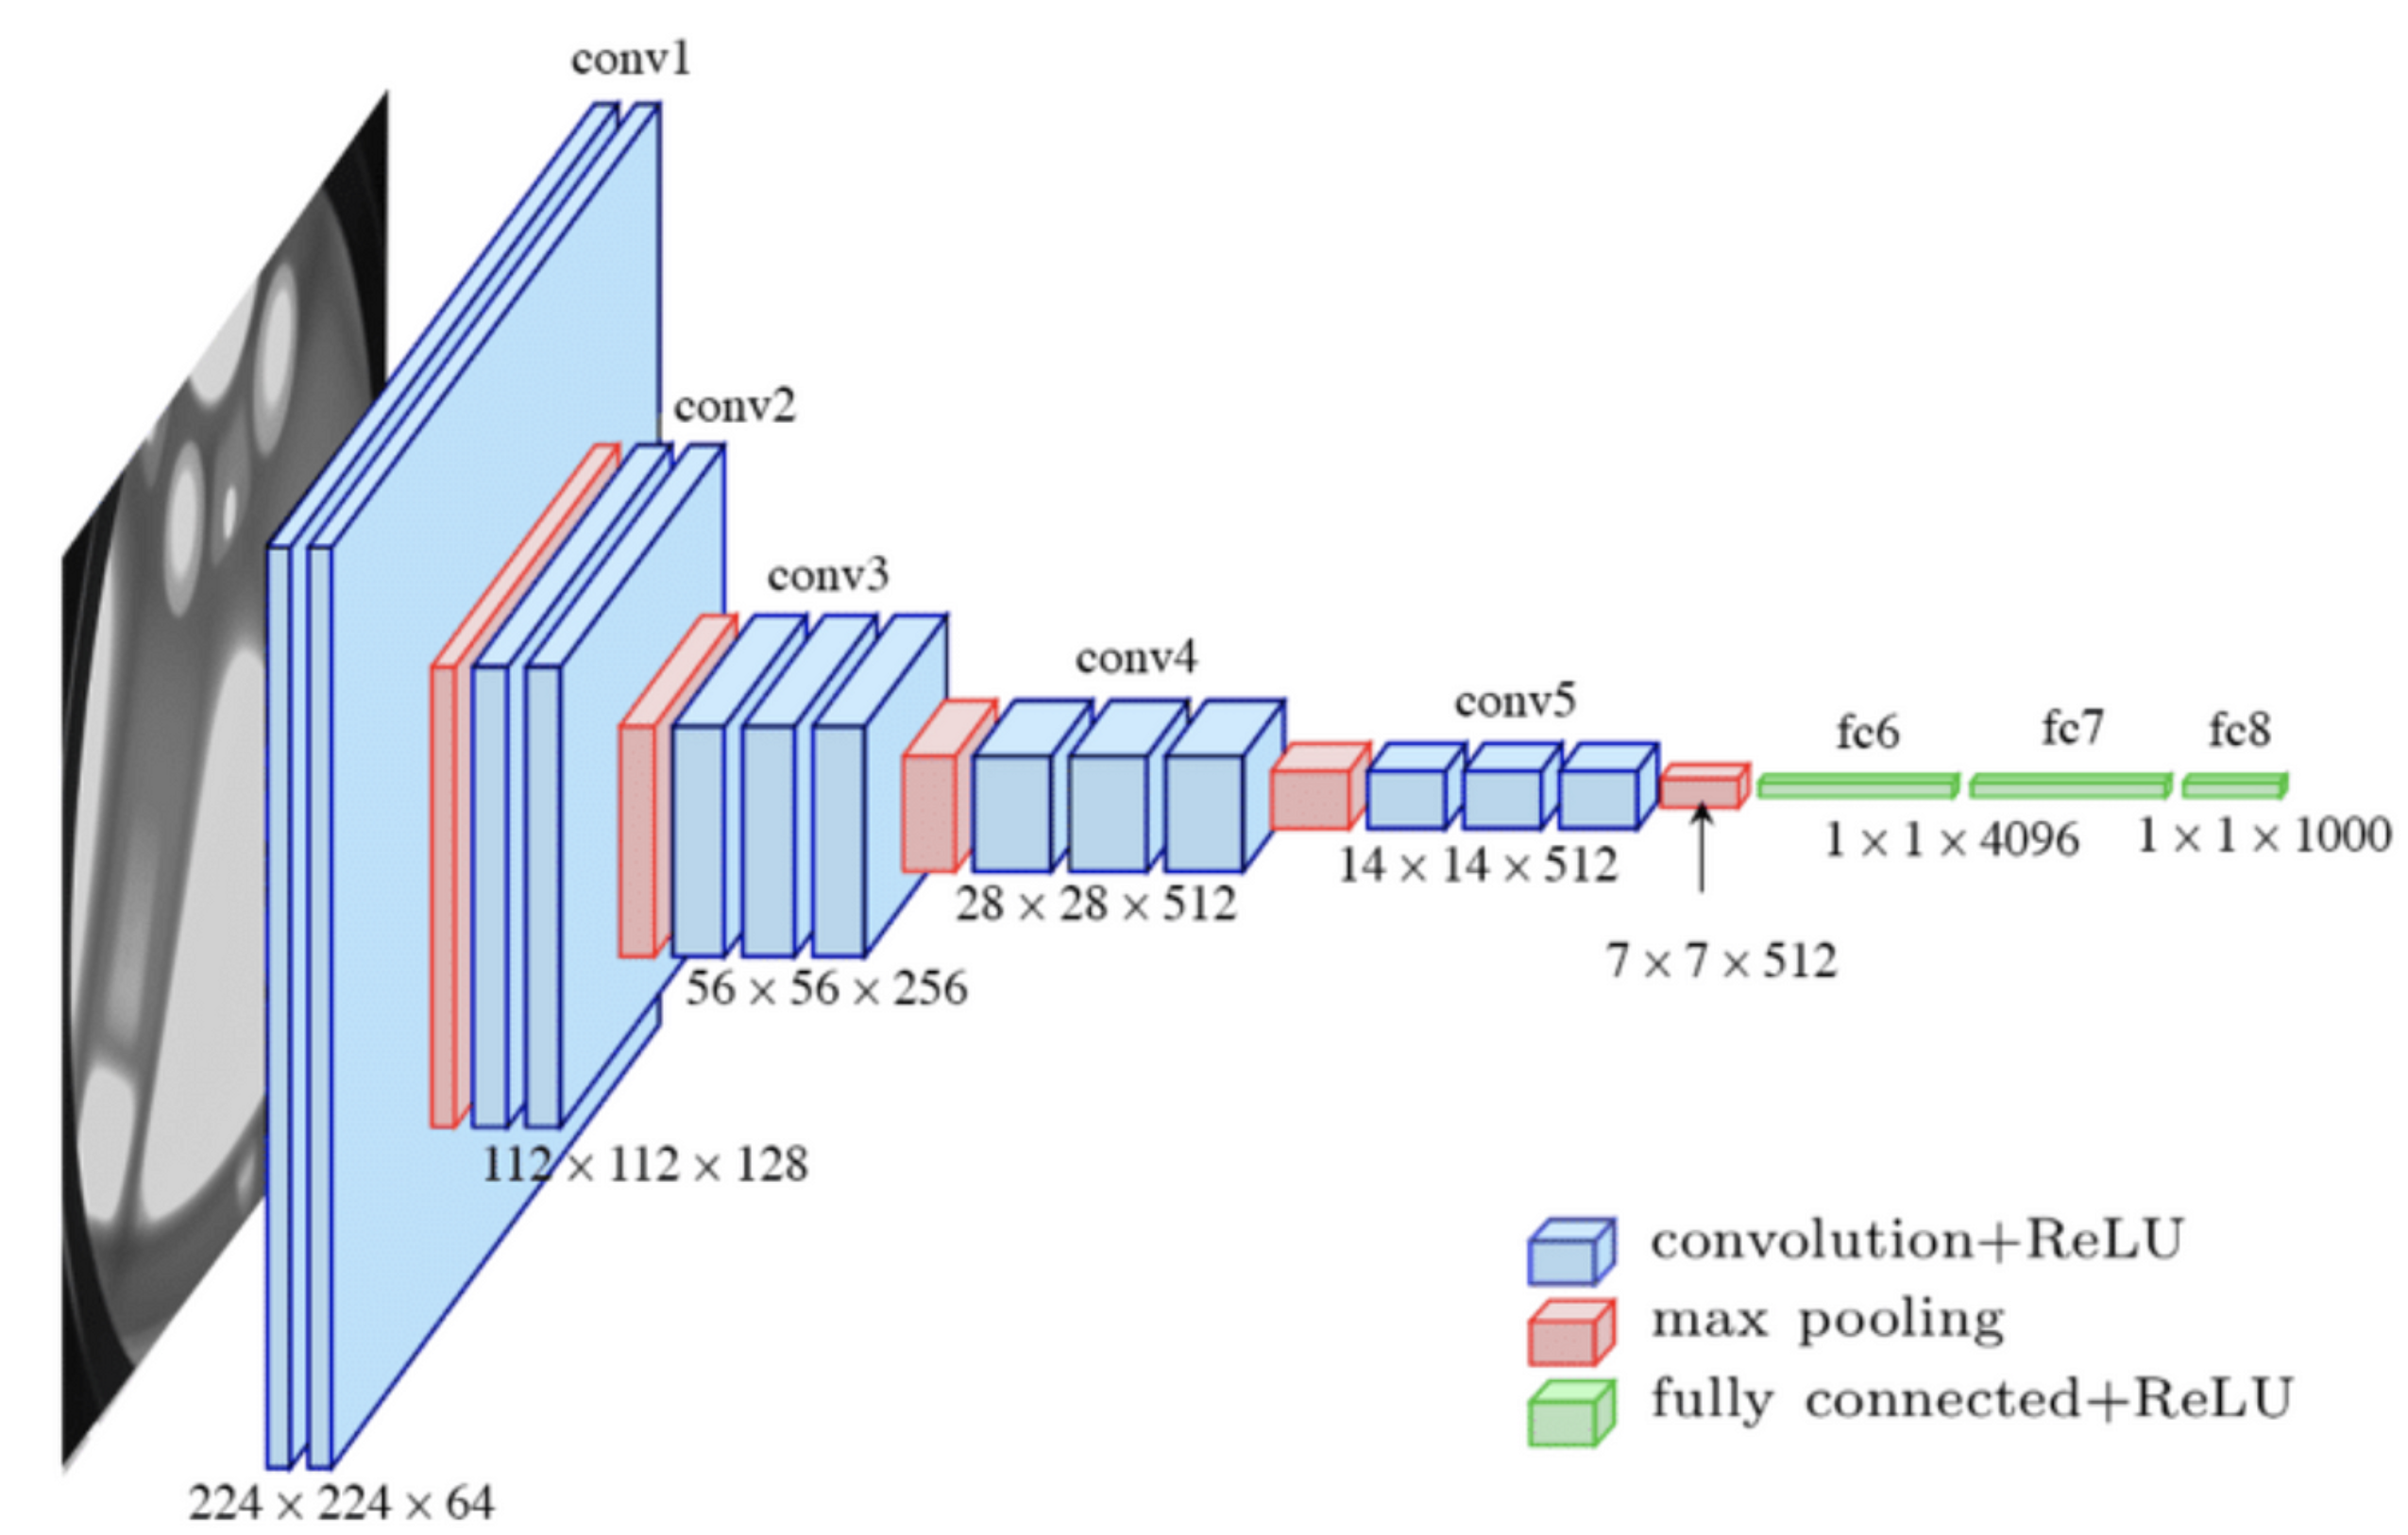
\includegraphics[height=6cm]{images/jcnn/vgg16.png}
  \caption{Graphic representation of the VGG-16 architecture, presenting the different kind of layer composing the architecture.}
  \label{fig:jcnn:vgg16}
\end{figure}

\begin{table}[ht]
  \centering
  \begin{tabular}{ | c | c | }
    \hline $N_{blocks}$ & {2, 3, 4} \\
    \hline $N_{channels}$ & {32, 64, 128} \\
    \hline
    \multirow{4}{*}{FCNN configuration} & 2 * 1024 \\
                                        & 2 * 2048 + 2 * 1024 \\
                                        & 3 * 2048 + 3 * 512 \\
                                        & 2 * 4096 \\
    \hline
    Loss & $E+V$, $E_r + V_r$ \\
    \hline

  \end{tabular}
\end{table}

\subsection{Data representation}
\label{jcnn:data}

\section{Results}

\begin{itemize}
  \item Comparison with victor results
  \item \textbf{More details when I'll look into the retrained data}
  \item Discuss of the differences
  \item Discuss of the principle of error decorelation
    \begin{itemize}
      \item Possible improvements
      \item Combining algorithms
      \item Average sum
    \end{itemize}
\end{itemize}

\section{Conclusion}
Intoduction next chapter
